% *******************************************************************************
% * Copyright (c) 2007 by Elexis
% * All rights reserved. This document and the accompanying materials
% * are made available under the terms of the Eclipse Public License v1.0
% * which accompanies this distribution, and is available at
% * http://www.eclipse.org/legal/epl-v10.html
% *
% *  $Id$
% *******************************************************************************
% !Mode:: "TeX:UTF-8" (encoding info for WinEdt)

\section{Kassenbuch}%\label{kassenbuch}
\index{Kassenbuch}
Elexis-Kassenbuch ist eine Minimalbuchhaltung zum Verbuchen von Bareinnahmen- und Ausgaben aus der Praxiskasse.

 Laden Sie das Kassenbuch-Plugin mit \href{http://www.rgw.ch/download.php?file=elexis-kassenbuch}{diesem Link} herunter und entpacken Sie das Archiv in Ihr Elexis-Verzeichnis. Starten Sie dann Elexis neu.
Fügen Sie die Kassenbuch-View durch Auswahl des Menüs Fenster-Ansicht-Andere... und dann Buchhaltung/Kassenbuch in die aktuelle Perspektive ein. Es erscheint folgende View:
\begin{figure}[htp]
\begin{center}
  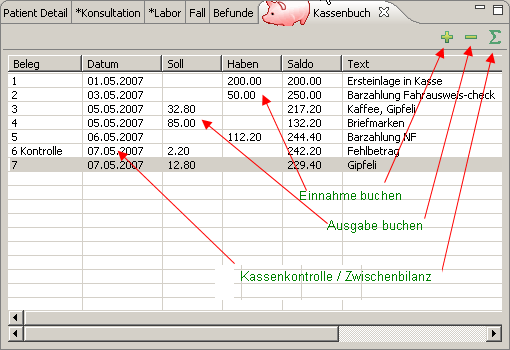
\includegraphics{images/kassenbuch}
  %\caption{Toolbar / Werkzeugleiste}
  \label{fig:kassenbuch}
\end{center}
\end{figure}

\begin{itemize}
 	\item Mit dem [+] - Icon können Einnahmen verbucht werden, mit dem [ - ]-  Icon Ausgaben.
	\item Das Summen-Icon dient dazu, die Buchhaltung mit dem tatsächlichen Kassenbestand abzugleichen (Zwischenbilanz). Wenn der Ist-Bestand niedriger ist, als der errechnete Bestand, dann wird die Differenz als Fehlbetrag gebucht, wenn er höher ist, als Überschuss. Eine Zwischenbilanz kann beliebig oft erstellt werden, und kann auch wieder gelöscht werden, wenn gewünscht.

	\item Mit Doppelklick auf eine Buchung, kann diese Buchung editiert werden.

	\item Mit Rechtsklick auf eine Buchung öffnet sich ein Kontextmenü zum Löschen der Buchung oder Zwischenbilanz.

	\item Die Belege werden nach der alphanumerischen Belegnummer sortiert. Diese sollte immer mit einer Zahl beginnen (wird auch automatisch so vorgegeben) und auf den entsprechenden Kassenbeleg geschrieben werden. Wenn nachträglich ein Beleg dazwischen eingefügt werden soll, kann man dies durch entsprechende Wahl der Belegnummer erreichen. Beispielsweise wird 2a zwischen 2 und 3 eingefügt.
\end{itemize}


